\documentclass[11pt]{article}
\usepackage{xspace}
\usepackage{times}
\usepackage{psfig}
\usepackage{amsmath}
\usepackage{graphicx}
\newcommand{\xorp} {{\em XORP}\@\xspace}
\newcommand{\module} {{\em module}\@\xspace}
\newcommand{\modules} {{\em modules}\@\xspace}
\newcommand{\finder} {{\em Finder}\@\xspace}
\newcommand{\xorpsh} {{\em Xorpsh}\@\xspace}
\newcommand{\cm} {{\em CM}\@\xspace}
\newcommand{\xrl} {{\em XRL}\@\xspace}
\newcommand{\rtrmgr} {{\em RTRMGR}\@\xspace}

\textwidth 6.5in
\topmargin 0.0in
\textheight 8.5in
\headheight 0in
\headsep 0in
\oddsidemargin 0in
%\date{}
\title{Error Handling in XORP}
%\author{Atanu Ghosh}
%\twocolumn
\begin{document}
\parsep 0ex
\parskip 1.0ex
\parindent 0em
\noindent
\maketitle                            
\section{Introduction}

A \xorp router is made up of a number processes that communicate via
XRLs \cite{xorp:xrl} (a messaging system developed for \xorp). In this
document we will focus on how to deal with errors that are generated
directly or indirectly by \xrl calls. As well as dealing with process
failure and restarts. Most \xorp processes share routing state that
must remain synchronised. For example, the BGP process sends the
result of its decision process to the RIB. If the RIB fails then BGP
has lost the ability to manipulate the FIB. BGP should either withdraw
all routes or more catastrophically drop all peerings until the RIB
restarts.

A critical component if the system is the \rtrmgr which is responsible
for starting and stopping routing processes. When a process is started
by the \rtrmgr or dies the \finder is notified. If a process has an
interest in the status of another process it can register interest
with the \finder.

In any complex system such as a \xorp router errors can occur. The
errors can range from a \xorp process failing to an attempt to install
a route that already exists. Errors will occur and need to be dealt
with in a consistent manor. The types of error that may occur are
categorised below.

The first type of error is {\em Proccess failure}.

The second type of error a {\em Communication Error}. At the most
basic level an attempt to send an \xrl has failed. The process that
was the recipient of the \xrl may have failed or be slow to respond.
The message that was being sent may have been lost in transit.

The third type of error {\em Execution Error} is when an an XRL call
returns an error due to some underlying interaction failure. The most
fundamental example of this type of error is a route add failing. The
attempt to add a route may fail for many reasons. The route may
already be present or a different route may be installed. The error
may occur due to a bug in the router code or because routing state has
been manipulated by non \xorp processes.

The fourth type of error {\em Type Error} is when an XRL call fails
because the arguments passed to an XRL are invalid. This error will
most likely be due to a version mismatch between \xorp processes. If
all the processes in a \xorp router have been built from the source
same tree this error should not occur. As we are building an
extensbile router it may be the case that a process built from a
different source tree may encounter compatibility problems.

\section{\label{pfailure}Process Failure}

A \xorp router is made up of a number of distinct processes. There are
dependencies between these processes. We define the critical
dependencies and what action to take on detecting failure.

The most critical component of a \xorp router is the \rtrmgr/\finder
process. One of the functions of this component is to start/re-start
processes. If process A is dependent on the status (alive, dead,
restarted) of process B, then process A registers this interest with
the \finder. This dependency on the \rtrmgr/\finder for managing and
monitoring process state mean that a \xorp router cannot survive the
failure of this process. A \xorp process on detecting the loss of the
\finder must exit. There is one exception to this rule the \xorpsh
process, this will be discussed later in section \ref{xorpsh}.

Each process in a \xorp router is described and how it should behave
when another process in the system fails. Processes can explicitly
register interest in the status of other processes through the
\finder. If process A is dependent on the state of process B then
process A must register interest in process B.

The only mechanism that a process should use to determine another
processes failure is notification from the \finder.

It is conceivable that the \finder could restart and in the same time
window another monitored process could restart. In which case the
restarting of the monitored process could be missed. To guard against
this possible race if the \finder fails or restarts all processes
should exit. The assumption is that the \finder failing is a very low
probability event.

\subsection{Implementing process failure detection}

The \finder process will send keepalive messages to all processes at
thirty second intervals. If a process does not respond to a keepalive
it is considered dead. The keepalive messages are sent over a reliable
transport such as TCP. A process dieing should therefore be easy to
detect. The \rtrmgr if it detects that a process has died will send a
hint to the \finder that will immediately try and send a keepalive.
Again if the process has died it should be easy to detect.

If a process is not responding to keepalives but it is still alive it
will be marked as dead and all interested processes will be notified.
Most importantly the \rtrmgr will be notified and it will kill the
running process and start a new process.

\subsection{Actions to take on detecting process failure}

Table \ref{failure_table} indicates what action a process should take
on detecting failure in other processes. The ``(G)'' denotes that the
process should attempt to exit gracefully. Figure \ref{failure_fig}
shows the relationship between the various processes. The thick arrows
should be modelled as a signal sent from a process dying to its
dependent processes.

\begin{figure}
  \begin{center}
    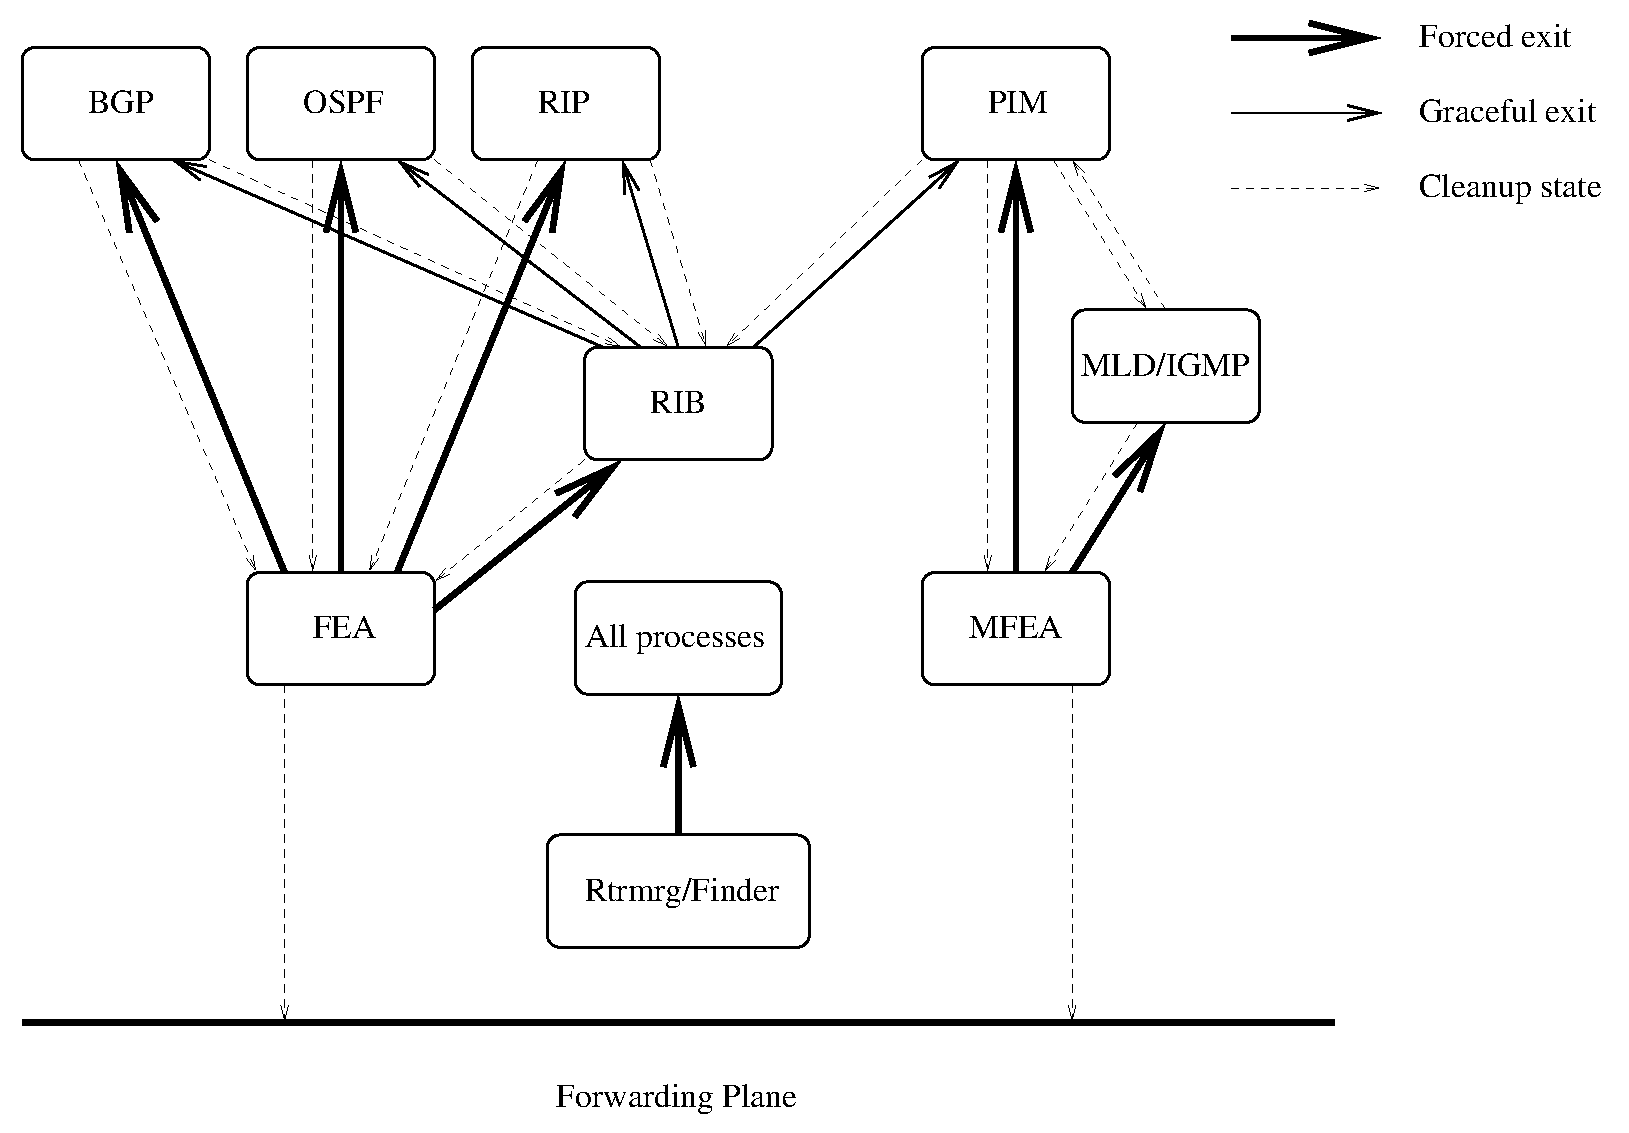
\includegraphics[width=0.9\textwidth]{figs/error_dependency.eps}
    \caption{Process relationship on failure}
    \label{failure_fig}
  \end{center}
\end{figure}

\begin{table}[ht]
\begin{center}
\begin{tabular}{|c|c|c|c|c|c|c|c|c|c|c|}
\hline
Process fails   &                 &          &      &      &      &         &      &      &      &         \\\hline
                & \rtrmgr/        & FEA      & MFEA & RIB  & IGMP & PIM     & BGP  & RIP  & OSPF & \xorpsh \\
                & \finder         &          &      &      &      &         &      &      &      &         \\\hline
\rtrmgr/        & /               & Withdraw & Exit & Exit & Exit & Exit    & Exit & Exit & Exit & Report  \\
\finder         &                 & All      &      &      &      &         &      &      &      & Problem \\
                &                 & Unicast  &      &      &      &         &      &      &      & Wait    \\
                &                 & Routes   &      &      &      &         &      &      &      &         \\
                &                 & Exit     &      &      &      &         &      &      &      &         \\\hline
FEA             &  Restart        & /        & Exit & Exit & Exit & Exit    & Exit & Exit & Exit & -       \\\hline
MFEA            &  Restart        & -        & /    & -    & Exit & Exit    & -    & -    & -    & -       \\\hline
RIB             &  Restart        & Withdraw & /    & -    & Exit & Exit    & Exit & Exit & Exit & -       \\
                &                 & All      &      &      & (G)  & (G)     & (G)  & (G)  & (G)  &         \\
                &                 & Unicast  &      &      &      &         &      &      &      &         \\
                &                 & Routes   &      &      &      &         &      &      &      &         \\\hline
IGMP            &  Restart        & -        & -    & -    & /    & Delete  & -    & -    & -    & -       \\
                &                 &          &      &      &      & Local   &      &      &      &         \\
                &                 &          &      &      &      & Members &      &      &      &         \\
                &                 &          &      &      &      & After   &      &      &      &         \\
                &                 &          &      &      &      & Timeout &      &      &      &         \\\hline
PIM             &  Restart        & -        & -    & -    & -    & /       & -    & -    & -    & -       \\\hline
BGP             &  Restart        & -        & -    & -    & -    & -       & /    & -    & -    & -       \\\hline
BGP             &  Restart        & -        & -    & -    & -    & -       & /    & -    & -    & -       \\\hline
RIP             &  Restart        & -        & -    & -    & -    & -       & -    & /    & -    & -       \\\hline
OSPF            &  Restart        & -        & -    & -    & -    & -       & -    & -    & /    & -       \\\hline
\xorpsh         &  Restart        & -        & -    & -    & -    & -       & -    & -    & -    & /       \\\hline
\end{tabular}
\end{center}
\caption{\label{failure_table}Action to take on detecting process failure}
\end{table}

\subsubsection{\rtrmgr/\finder - Router manager}

If the \rtrmgr/\finder dies then all bets are off and all processes
should exit apart from the \xorpsh.

If a \xorp process exits unexpectedly the \rtrmgr/\finder should
attempt to restart the process.

\subsubsection{FEA - Forwarding Engine Abstraction}

The FEA primarily excepts routes from the RIB and places them in the
kernel. The FEA should tag all routes that it has installed in the
kernel. The FEA on restart should remove all routes that a previous
incarnation of the FEA has placed in the kernel. When an FEA is
exiting it should attempt remove all routes that it has installed in
the kernel.

The FEA process should register interest in the RIB. If the RIB fails
the FEA should withdraw all routes that the RIB has sent to it.

\subsubsection{MFEA - Multicast Forwarding Engine Abstraction}

The MFEA is multicast analogue to the unicast FEA. If should be noted
that the MFEA and FEA are currently being merged.

\subsubsection{RIB - Routing Information Base}

Routes from the routing processes are sent to the RIB the winners are
sent to the FEA.

The RIB should register interest in the FEA. If the FEA fails the RIB
should exit. All routing processes that interact with the RIB should
on detecting the shutdown of the RIB also terminate gracefully.

\subsubsection{IGMP/MLD}

If the FEA/MFEA process exits then this process should exit.

\subsubsection{PIM}

If the RIB or FEA/MFEA exits then this process should exit.

\subsubsection{BGP}

Currently the only other process in the system that the RIB interacts
with is the RIB. If the BGP process detects that the RIB has died then
it should gracefully terminate its sessions and exit.

In the future the TCP connections that BGP makes will be mediated
through FEA. At which time the BGP process should also register
interest in the state of the FEA. If the BGP process detects the death
of the FEA it should exit immediately.

\subsubsection{RIP}

The RIP process should register interest in the FEA and the RIB. If
the RIB dies then the RIP process should attempt to exit gracefully.
If the FEA dies the RIP process should exit immediately.

\subsubsection{IS-IS}

The IS-IS process should register interest in the FEA and the RIB. If
the RIB dies then the IS-IS process should attempt to exit gracefully.
If the FEA dies the IS-IS process should exit immediately.

\subsubsection{OSPF}

The OSPF process should register interest in the FEA and the RIB. If
the RIB dies then the OSPF process should attempt to exit gracefully.
If the FEA dies the OSPF process should exit immediately.

\subsubsection{\label{xorpsh}\xorpsh}

The \xorpsh provides a command line interface to the XORP router.
Other processes in the system exiting should never cause it to
exit. The \rtrmgr/\finder process exiting should generate
warning output to the user and then the \xorpsh should wait for the
router to restart.

\section{XRL Communication Error}
Interprocess communication in \xorp is achieved using XRLs. In this
section we will consider what should be done when an XRL call fails
due to a communication error.

All XRL calls will ultimately get a response. In the normal case the
response returns the status of the call (good or bad). In addition to
error responses produced by the application, the XRL library can also
return the following error responses:
\begin{itemize}
\item NO\_FINDER
\item RESOLVE\_FAILED
\item SEND\_FAILED
\item REPLY\_TIMED\_OUT
\item FATAL\_TRANSPORT\_ERROR
\end{itemize}
From an application point or view, the first three errors are
equivalent: the XRL was not communicated to the destination.  We will
discuss these below using the generic term {\em XRL send failure}.

XRLs can be sent over unreliable transports such as UDP or reliable
transports such as TCP. The type of transport that should be used will
be specified when defining the interface. In the case of reliable
transport, the errors above should generally not occur, but in any
event we need general rules about how to handle them should something
fail in an unexpectedly way.

In the case of an unreliable transport, REPLY\_TIMED\_OUT may be
expected, but 
\newline
FATAL\_TRANSPORT\_ERROR will never occur.  In the case
of a reliable transport, FATAL\_TRANSPORT\_ERROR may occur, but
REPLY\_TIMED\_OUT will never occur.

It's not clear what can be inferred from a timeout response. The
reasons for a timeout might be: the peer has died, peer is slow to
respond, the network cable has been removed. As in all network
communications when a timeout occurs we don't know if the last
unacknowledged XRL request was received and processed by the peer.

If the timeout has occurred because the peer has died we will receive
notification of this explicitly and will deal with it as specified in
section \ref{pfailure}.  Thus an XRL transport error SHOULD NOT be
taken as an indication that the peer is dead.  If an application cares
that the peer has died or restarted, it SHOULD register with the
finder to receive notifications of process restarts.  This a process
SHOULD assume that an XRL transport problem will be transient until it
receives an explicit confirmation that the destination has failed. 

In addition, to an XRL interface being reliable or unreliable, the way
the application uses an XRL interface can by pipelined or
non-pipelined.  In the pipelined case, multiple requests can be
outstanding simultaneously; in the non-pipelined case at most one
request can be outstanding at a time.

It is useful for us to categorise XRL interfaces along these two axes:
reliable/unreliable and pipelined/non-pipelined.

\subsection*{Unreliable, Non-pipelined}

If an XRL send failure occurs, the sending application MAY choose to
retransmit the XRL, or ignore the failure as it sees fit.  

In an XRL timeout occurs, the sending application MAY also choose to
retransmit the XRL, or ignore the failure as it sees fit.  However, if
the application chooses to re-send the XRL, the interface MUST be
written in such a way that if this XRL had previously been received,
this will not cause a further failure.

\subsection*{Reliable, Non-pipelined}

If an XRL send failure occurs, the sending application SHOULD
retransmit the XRL.  Further requests using this interface
MUST be queued until the XRL has successfully been received.

If a FATAL\_TRANSPORT\_ERROR occurs, this is an unrecoverable error.
The application should cause this XRL interface to go dormant, in the
expectation that it will authoritatively discover from the finder that
the target has died.

\subsection*{Unreliable, Pipelined}

The same issues apply as with unreliable, non-pipelined, but the
situation is more complicated.  An interface that uses unreliable
transport and pipelining is one that explicitly permits loss and {\em
re-ordering} of requests.  It is up to the application to choose
whether to retransmit XRLs that return XRL send failed or timeout, but
the application must only do so if it is certain that the re-ordering
caused by retransmission will not be a problem.

\subsection*{Reliable, Pipelined}

Reliable, pipelined interfaces are the most difficult in which to
handle XRL errors.  In the general case, three issues would need to be
considered:
\begin{itemize}
\item The XRL that failed due to a transport error may be followed by
pipelined XRLs that succeeded.
\item The XRL that failed due to a transport error may be followed by
pipelined XRLs that failed at the application level due to the state
caused by the first failed XRL not being instantiated.
\item If a failed XRL was followed by pipelined XRLs that succeeded,
retransmitting that XRL will cause a re-ordering that might leave the
destination in a different state than it would be if the XRLs had
arrived in order.
\end{itemize}
To avoid the need to consider all these problems we require that a
reliable XRL transport fail to deliver all subsequent XRLs in the
pipeline if a single XRL fails.

Thus, in the case of an XRL send error, the reliable pipelined
interface SHOULD fall back to a reliable, non-pipelined behaviour
after a failure, and SHOULD retransmit the first XRL that failed until
either it is successful or the application authoritatively discovers
from the finder that the target has died.  After the retransmitted XRL
is successful, the pipelined operation may resume.

If a FATAL\_TRANSPORT\_ERROR occurs, this is an unrecoverable error.
The application SHOULD cause this XRL interface to go dormant, in the
expectation that it will authoritatively discover from the finder that
the target has died.

\section{Execution Error}

A XORP router is partitioned into many processes most of the operating
system specific interactions are performed by the FEA. In a router the
most frequent operation will be the adding and deleting of routes.
Consider BGP adding a route; first the BGP process will send the route
to the RIB, then the route may be sent to FEA. If the addition of the
route from the RIB to the FEA fails then there is no way of
propogating this failure back to the BGP process due to the
asynchronous nature of XRLs. If adding/deleting a route fails a very
drastic way of propogating this failure back to the BGP process would
be for either or both the FEA and RIB processes to exit. If which case
the process failure responses already described would be used and BGP
would exit. Processes exiting would be an extreme response to failing
to add a route because it already exists. It is important though not
to mask over implementation problems by ignoring errors. In the rest
of this section we will outline how to deal with a number of common
errors.

\subsection{Adding/Deleting route failures}

As stated above a highly likely error could failures when adding or
deleting routes. Typically the interaction will occur between the RIB
and FEA. When an error occurs it should be logged by the FEA and the
cause be returned to the RIB. The RIB can be configured with policy on
how to react to different errors.

Adding a route will typically fail because a route already exists.
Firstly, if a route already exists it is either the same or different
to the one that we attempted to add. Secondly, either the FEA
installed the route or a third party installed it. Therefore when
adding a route fails the FEA should return if the current route is the
same or different to the one we attempted to add as well as who
installed the route originally. The RIB on receiving the error state
from the FEA can decide as a matter of policy how to proceed. If an
attempt to add a route fails because a different route exists the RIB
could choose to delete the old route and add the new route.

The most common reason for a route deletion to fail would be that the
route is no longer present. The FEA should log that it has been asked
to delete a route that doesn't exist. The RIB should decide if this
problem should be considered fatal.


%%%%%%%%%%%%%%%%%%%%%%%%%%%%%%%%%%%%%%%%%%%%%%%%%%%%%%%%%%%%%%%%%%%%%%%
%     BIBLIOGRAPHY
%%%%%%%%%%%%%%%%%%%%%%%%%%%%%%%%%%%%%%%%%%%%%%%%%%%%%%%%%%%%%%%%%%%%%%%
\bibliography{../tex/xorp}
\bibliographystyle{plain}

%%%%%%%%%%%%%%%%%%%%%%%%%%%%%%%%%%%%%%%%%%%%%%%%%%%%%%%%%%%%%%%%%%%%%%%
\end{document}
